\newpage
\section{Amplificadores de transconductancia (OTA)}
\subsection*{Introducción}
Los amplificadores de transconductancia integrados se comportan como fuentes de corriente controladas por tensión, siendo obviamente el parámetro de transferencia, la transconductancia ($g_m$). Desde este punto de vista emulan el comportamiento de los transistores discretos, mostrando modelos lineales equivalentes semejantes aunque con mucho más refinamiento en la precisión y control de sus parámetros.

Existen dos tipos bien diferenciados según se deriven de la arquitectura de amplificadores VFA o CFA, no obstante ambos estructuralmente tienen solo dos etapas, una primera diferencial cuya corriente es reproducida a la salida por la segunda, que se corresponde con un espejo de corriente. A diferencia de los dos tipos de amplificadores estudiados previamente estos pueden operar linealmente sin realimentación (Amplificación Directa), teniendo en esta modalidad excelente performance en altas frecuencias debido al reducido número de etapas que poseen.
\subsection{OTA-VFA}
Este tipo utiliza la etapa de entrada del diferencial clásico de los VFA, con versiones comerciales de tecnología Bipolar o MOS, en consecuencia presentan muy alta impedancia en los dos terminales de entrada y alta en el de salida. La figura \ref{fig:4.1}, muestra el símbolo frecuentemente utilizado y el modelo lineal equivalente en bajas frecuencias.
\begin{figure}[H]
    \centering
    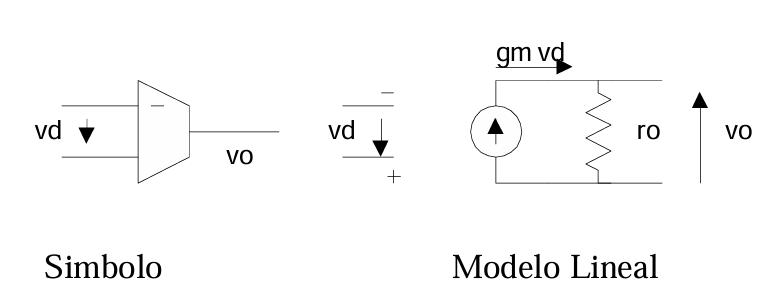
\includegraphics[width=0.5\linewidth]{Imagenes/4.1.png}
    \caption{}
    \label{fig:4.1}
\end{figure}
La transconductancia ($g_m$) del conjunto se corresponde con la del diferencial de entrada y es función directa de la corriente de polarización del mismo que puede ser variada externamente por tensión dentro de los límites especificados en la hoja de datos respectiva.

\begin{equation}
g_m = \frac{I_0}{2 V_t}
\label{eq:4.1}
\end{equation}

$I_0 = \text{Corriente de polarización}$

El modo diferencial máximo depende del grado de distorsión admitida, para una etapa diferencial bipolar simple no supera los $2V_t$ ($\cong \pm 50\,\text{mV}$ a $25\,^\circ\text{C}$), este rango puede ser ampliado al orden del voltio, con el agregado de diodos de linealización a la entrada, que además compensan térmicamente la transconductancia cuando los diodos están integrados al chip. En la actualidad la mayoría de las versiones comerciales los tienen incorporado.
\subsubsection{Aplicaciones}
La posibilidad de ajuste externo del parámetro de transferencia $g_m$ mediante la corriente de polarización, hace que este tipo de amplificadores encuentren amplio campo de aplicación, en la realización de circuitos eléctricamente sintonizables, tales como amplificadores de ganancia controlada, osciladores y filtros activos. A continuación se analizarán algunas de las aplicaciones típicas comentadas.

\textbf{Amplificador Directo}

El OTA puede ser utilizado como amplificador de tensión directo o en configuraciones realimentadas. En el primer caso Fig \ref{fig:4.2}, la ganancia de tensión puede ser ajustada externamente a través de la transconductancia $g_m$ (\ref{eq:4.2})

\begin{equation}
A_v = g_m . Z_L
\label{eq:4.2}
\end{equation}

\begin{figure}[H]
    \centering
    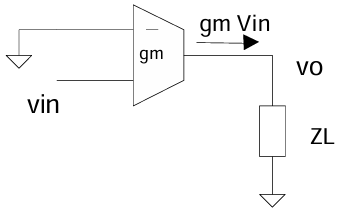
\includegraphics[width=0.5\linewidth]{Imagenes/4.2.png}
    \caption{Amplificador directo de ganancia controlada}
    \label{fig:4.2}
\end{figure}
\subsubsection{Configuraciones realimentadas}
Las configuraciones realimentadas negativamente son muy utilizadas para simular componentes pasivos, tales como resistores e inductores eléctricamente sintonizables. Por ejemplo la configuración de figura \ref{fig:4.3} se comporta en bajas frecuencias como una resistencia con un extremo a tierra, de valor inverso a la transconductancia del OTA ($r_m=1/g_m$).

En efecto asumiendo el modelo de fig \ref{fig:4.1}, en términos idealizados ($r_i = r_o = \infty$), se deduce por simple inspección la siguiente relación para la impedancia de entrada.

\begin{equation}
Z_{in} = \frac{V_{in}}{I_{in}} = \frac{V_{in}}{g_m V_{in}} = \frac{1}{g_m} = r_m
\label{eq:4.3}
\end{equation}
\begin{figure}[H]
    \centering
    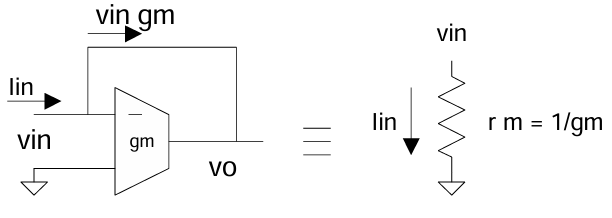
\includegraphics[width=0.85\linewidth]{Imagenes/4.3.png}
    \caption{Resistencia a tierra}
    \label{fig:4.3}
\end{figure}
\subsection*{Ejemplo 4.1}
\noindent\rule{\textwidth}{0.4pt}

\vspace{0.2cm}
\noindent Analizar el efecto de la impedancia de salida finita, sobre el valor idealizado, dado por (\ref{eq:4.3}).
\vspace{0.2cm}

\noindent\rule{\textwidth}{0.4pt}

\vspace{0.2cm}
\noindent Para el análisis propuesto se utilizará la fórmula de Blackman, con el circuito modelado como lo muestra la figura \ref{fig:4.4}, de la que se deducen las GL respectivas ($T_{cc}$ y $T_{ca}$).
\begin{figure}[H]
    \centering
    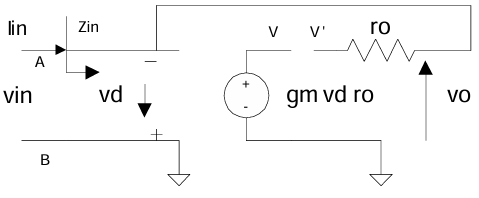
\includegraphics[width=0.65\linewidth]{Imagenes/4.4.png}
    \caption{Impedancia del sistema muerto}
    \label{fig:4.4}
\end{figure}
$$
Z_{in}|_{V'=0} = \frac{V_{in}}{I_{in}} = r_O
$$

Es fácil ver que la ganancia de lazo para la sección de interés (A-B), en cortocircuito es nula debido a que:

$$
v_d = 0 \Rightarrow v = 0 \hspace{3cm} T_{cc} = \left( \frac{v}{v'} \right) \bigg|_{vin=0} = 0
$$

En cambio para la sección abierta es $v_d = v'$, luego:

$$
T_{ca} = \left( \frac{v}{v'} \right) \bigg|_{Iin=0} = -g_m \cdot r_O
$$

Finalmente

$$
Z_{if} = \frac{r_O}{(1+g_m \cdot r_O)}
$$

En la anterior se ve que si $r_O \to \infty \Rightarrow Z_{in} \to 1/g_m$
La configuración un tanto más compleja de fig \ref{fig:4.5}, logra simular un resistor flotante, cargando entrada y salida del OTA ($O_1$), con resistencias a tierra iguales, simuladas por ($O_2$) y ($O_3$), respectivamente.

En efecto en el nudo de entrada se cumple

\begin{equation}
I_{in} = -(V_O - V_{in}) \cdot g_m \rightarrow \frac{(V_{in} - V_O)}{I_{in}} = \frac{1}{g_m} = r_m
\label{eq:4.4}
\end{equation}

Tomando el circuito como un súper nodo se deduce la impedancia vista desde el nodo $V_O$.

\begin{equation}
I_{in} = -I_O \Rightarrow \frac{(V_O - V_{in})}{I_O} = \frac{1}{g_m} = r_m
\label{eq:4.5}
\end{equation}

\begin{figure}[H]
    \centering
    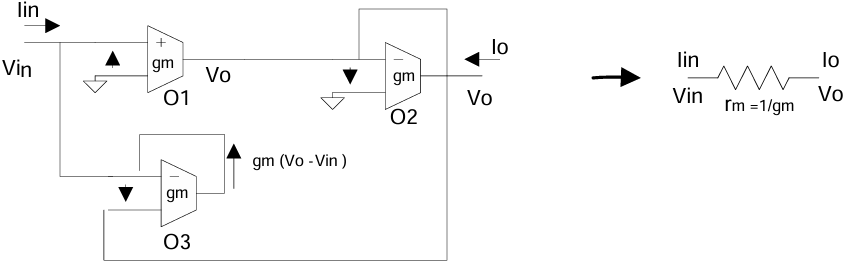
\includegraphics[width=0.65\linewidth]{Imagenes/4.5.png}
    \caption{Resistor flotante}
    \label{fig:placeholder}
\end{figure}

El circuito anterior cargado con un capacitor, genera una sección de filtro pasabajos de primer orden, cuya frecuencia de corte puede ajustarse eléctricamente a través de $g_m$.
\begin{figure}[H]
    \centering
    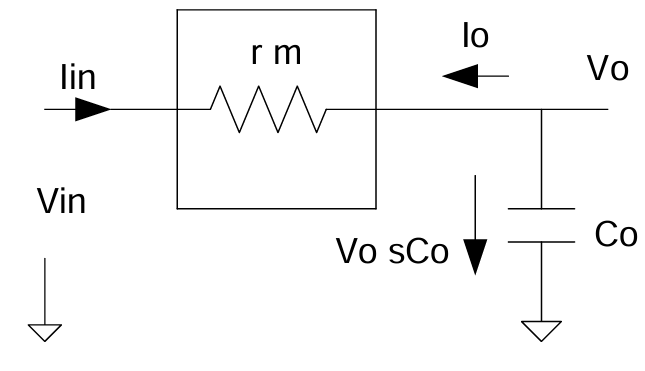
\includegraphics[width=0.5\linewidth]{Imagenes/4.6.png}
    \caption{Sección pasabajos R-C}
    \label{fig:placeholder}
\end{figure}
En efecto a partir de figura \ref{fig:4.6}, donde el bloque $r_m$ representa al circuito de figura \ref{fig:4.5}, se deduce la siguiente función de transferencia.
\begin{equation}
I_O = \frac{(V_O - V_{in})}{r_m} = -V_O \cdot s \cdot C \quad \rightarrow \quad A_v(s) = \frac{V_O}{V_{in}} = \frac{1}{(1 + s \cdot C \cdot r_m)}
\label{eq:4.6}
\end{equation}

Se denominan \textit{giradores} a aquellos circuitos que muestran una impedancia de entrada que es la inversa de la de carga. Esta transformación permite simular inductores, cargando un girador con un capacitor. La conexión OTA de figura \ref{fig:4.7} es un ejemplo y de ella se deducen las siguientes relaciones.

\begin{figure}[H]
    \centering
    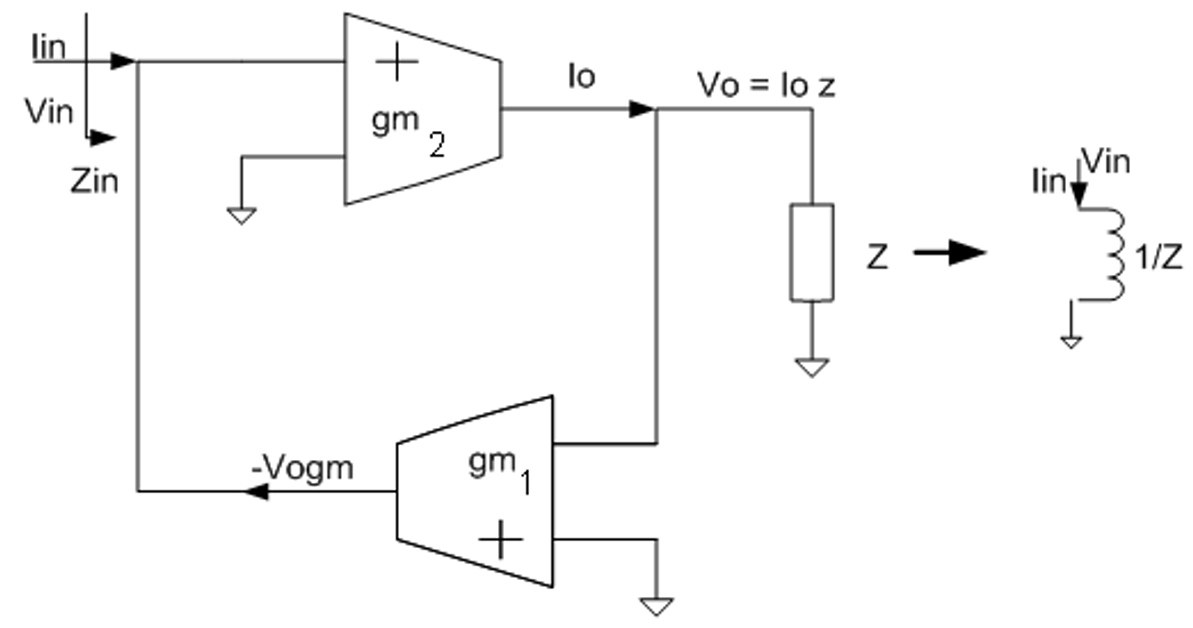
\includegraphics[width=0.5\linewidth]{Imagenes/4.7.png}
    \caption{Girador(inductor a tierra)}
    \label{fig:placeholder}
\end{figure}
\begin{equation}
I_{in} = V_O \cdot g_{m1} = V_{in} \cdot g_{m1} \cdot Z \cdot g_{m2} \quad \Rightarrow \quad \frac{V_{in}}{I_{in}} = \frac{1}{g_{m1} \cdot g_{m2} \cdot Z}
\label{eq:4.6}
\end{equation}

Si $Z = \frac{1}{s \cdot Cx} \Rightarrow Z_{in} = s \cdot \left( \frac{Cx}{g_{m1} \cdot g_{m2}} \right) = s \cdot Lx \quad \text{donde:} \quad Lx = \left( \frac{Cx}{g_{m1} \cdot g_{m2}} \right)$
\begin{equation}
\label{eq:4.7}
\end{equation}

La conexión de dos giradores similares al de figura \ref{fig:4.7} excitando en contrafase la impedancia $Z$ (Fig \ref{fig:4.8}), simulan un inductor flotante conectado entre entrada y salida, cuando aquella es un capacitor.

$$
Vx = (V_O \cdot g_{m1} - V_{in} \cdot g_{m1}) \cdot Z
$$

Si $Z = \frac{1}{s \cdot Cx}$ e $I_{in} = -Vx \cdot g_{m2} \Rightarrow Z_{in} = \left( \frac{V_{in} - V_O}{I_{in}} \right) = \left( \frac{s \cdot Cx}{g_{m1} \cdot g_{m2}} \right)$
\begin{equation}
\label{eq:4.8}
\end{equation}

De igual manera la impedancia vista desde el otro extremo será:

$$
I_{in} = -I_O \quad \Rightarrow \quad Z_0 = \left( \frac{V_O - V_{in}}{I_0} \right) = s \cdot Lx
$$
\begin{figure}[H]
    \centering
    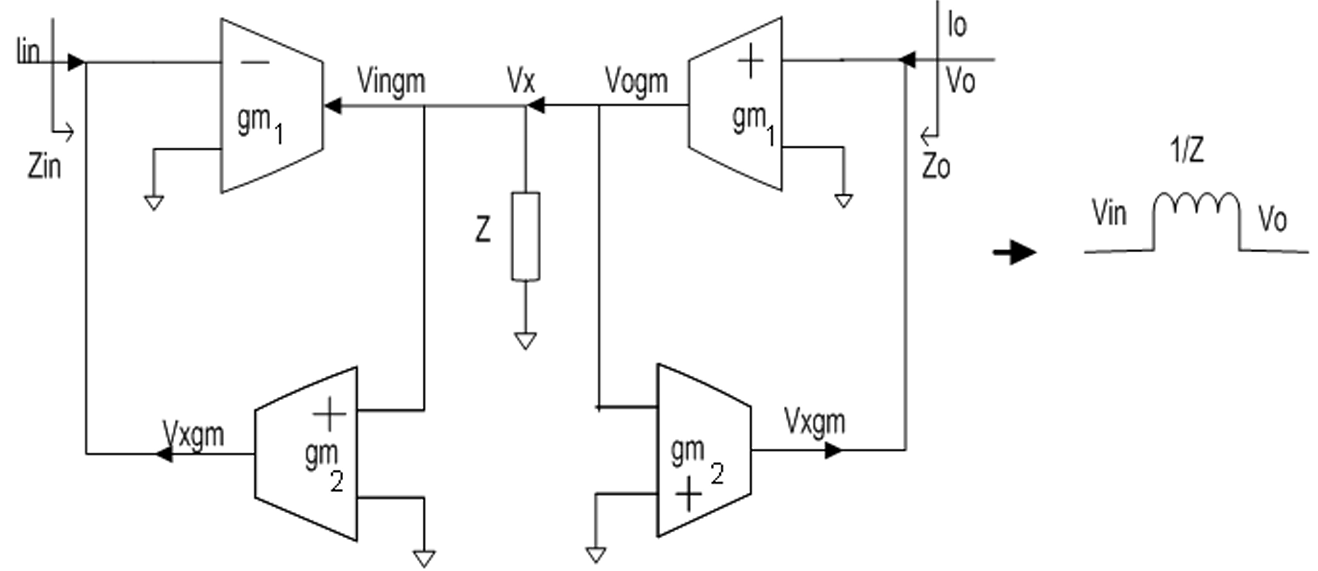
\includegraphics[width=0.65\linewidth]{Imagenes/4.8.png}
    \caption{Inductor flotante}
    \label{fig:4.8}
\end{figure}
Cargando la salida del inductor flotante de figura \ref{fig:4.8}, con un capacitor, se genera una sección pasabajos de segundo orden no disipativa ($L-C$).

En efecto en referencia a la figura \ref{fig:4.9} y a partir de la ecuación (\ref{eq:4.8}), se deduce la función de transferencia respectiva.

\begin{equation}
\text{Siendo: } I_0 = -V_0 \cdot s \cdot C_0 = \frac{(V_0 - V_{in})}{s \cdot Lx} \quad \Rightarrow \quad \frac{V_0}{V_{in}} = \frac{1}{Lx \cdot C_0} \cdot \frac{1}{\left( s^2 + \frac{1}{Lx \cdot C_0} \right)}
\end{equation}

\begin{figure}[H]
    \centering
    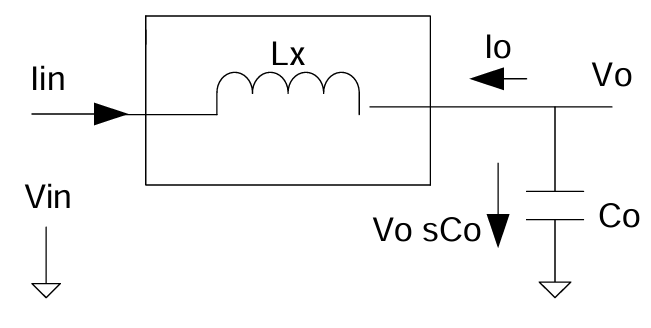
\includegraphics[width=0.5\linewidth]{Imagenes/4.9.png}
    \caption{Sección pasabajos L-C}
    \label{fig:4.9}
\end{figure}
Las versiones comerciales de estos integrados incluyen en el mismo chip un Buffer que permite ampliar el campo de aplicaciones posibles. Por ejemplo se puede configurar un amplificador operacional clásico, por la conexión en cascada de ambos (fig \ref{fig:4.10}). Obviamente la elevada impedancia de entrada del buffer ($Z_{inb}$), mueve en el mismo sentido la ganancia de tensión del conjunto ($A_v = g_m \cdot Z_{inb}$), obligando a que sus aplicaciones se limiten a configuraciones realimentadas.

\begin{figure}[H]
    \centering
    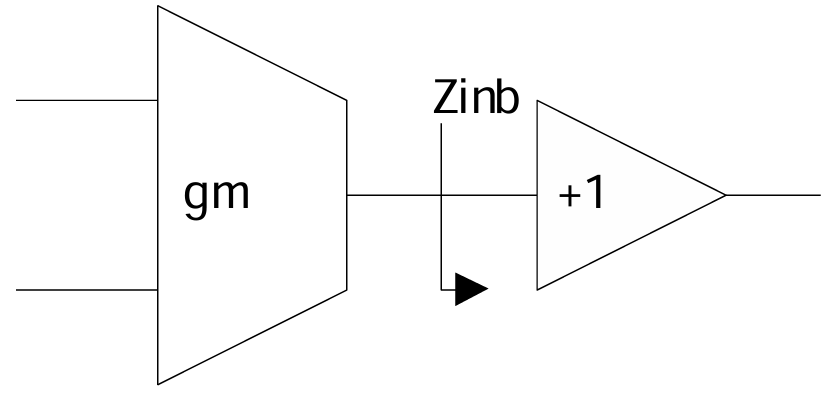
\includegraphics[width=0.5\linewidth]{Imagenes/4.10.png}
    \caption{}
    \label{fig:4.10}
\end{figure}

\subsection{OTA-CFA (transistor diamante)}
Esta segunda versión de amplificadores OTAs, denominada por sus diseñadores (Burr-Brown Corp), como Fuente de Corriente Diamante (DCS) o también Transistor Diamante (DT) se deriva de la arquitectura bipolar CFA y utiliza la misma etapa diferencial de entrada (Buffer Diamante), en consecuencia la impedancia de entrada del terminal no inversor, denominada Base del transistor Diamante, es muy elevada y en cambio la del inversor (Emisor del TD) muy baja. Ambos emulan una junta cuya relación corriente de emisor-tensión de control resulta lineal y bidireccional (Fig. \ref{fig:4.11}). El rango de modo diferencial máximo admitido con mínima distorsión se corresponde no obstante con el diferencial clásico, es decir aproximadamente $\pm 50\,\text{mV}$.
\begin{figure}[H]
    \centering
    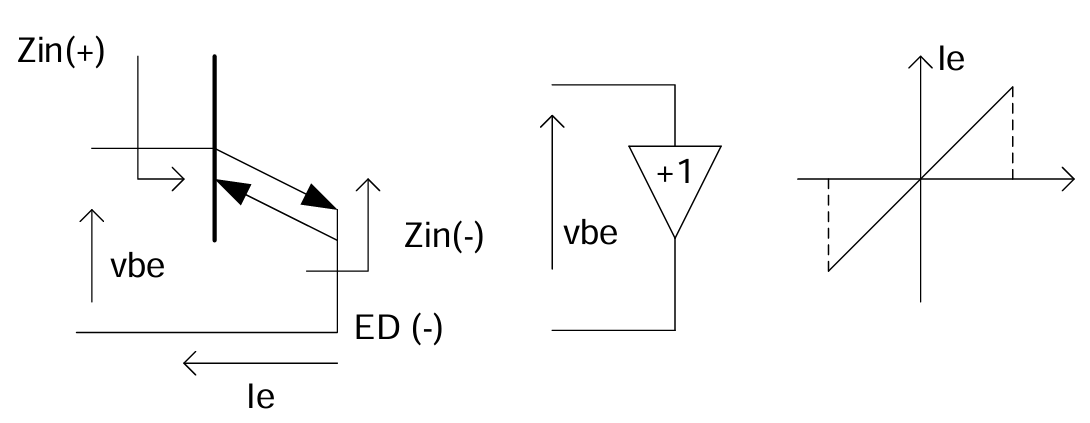
\includegraphics[width=0.5\linewidth]{Imagenes/4.11.png}
    \caption{}
    \label{fig:4.11}
\end{figure}
La etapa de salida vuelve a ser un espejo de corriente que en este caso copia con relación 1/1, la corriente del emisor cuya salida configura el colector equivalente ($C_d$), con una impedancia asociada del mismo orden de magnitud que el caso clásico.

La fig. \ref{fig:4.12}a, muestra el símbolo frecuentemente utilizado para representarlo, la doble flecha recuerda su característica bidireccional en términos de corriente total en sus terminales, y en fig \ref{fig:4.12}b el modelo en baja frecuencia. En virtud de que la corriente de colector reproduce en módulo y sentido la de emisor, la característica de transferencia de la fig. \ref{fig:4.11} se extiende a la corriente de colector.
\begin{figure}[H]
    \centering
    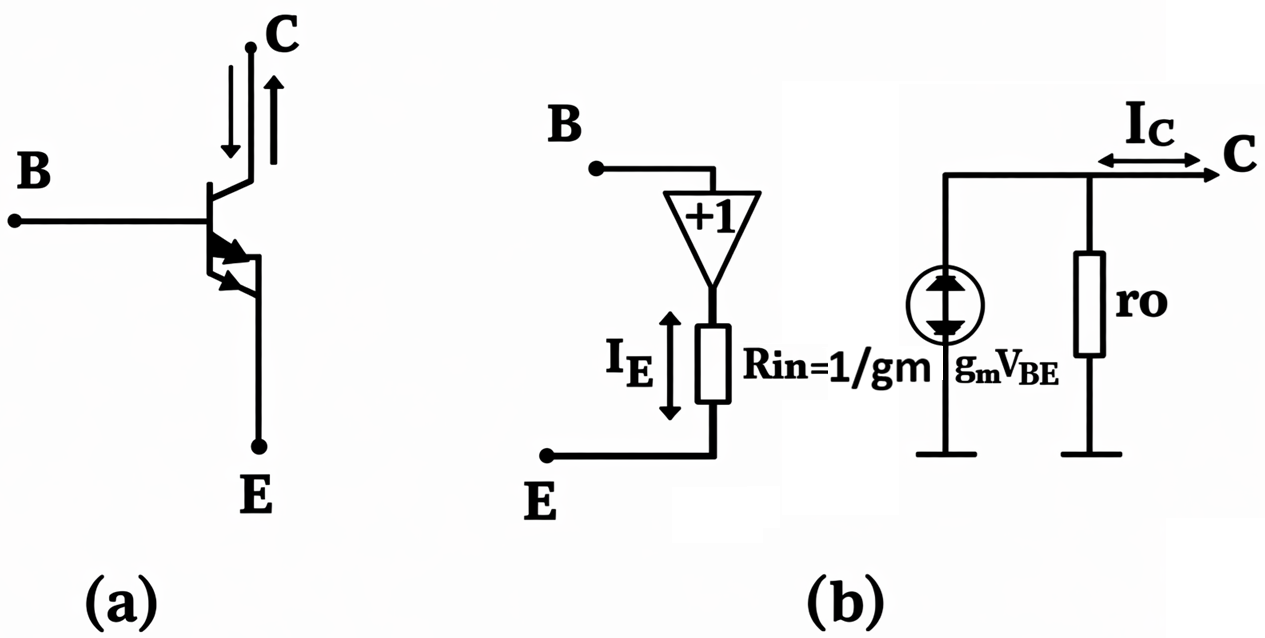
\includegraphics[width=0.5\linewidth]{Imagenes/4.12.png}
    \caption{}
    \label{fig:4.12}
\end{figure}
La fig. \ref{fig:4.13}, extiende y cuantifica los conceptos desarrollados mostrando un cuadro de características y parámetros comparativo con los dos elementos discretos de juntura, (JFET y BJT), que operan como fuentes de corriente controlada.
\begin{figure}[H]
    \centering
    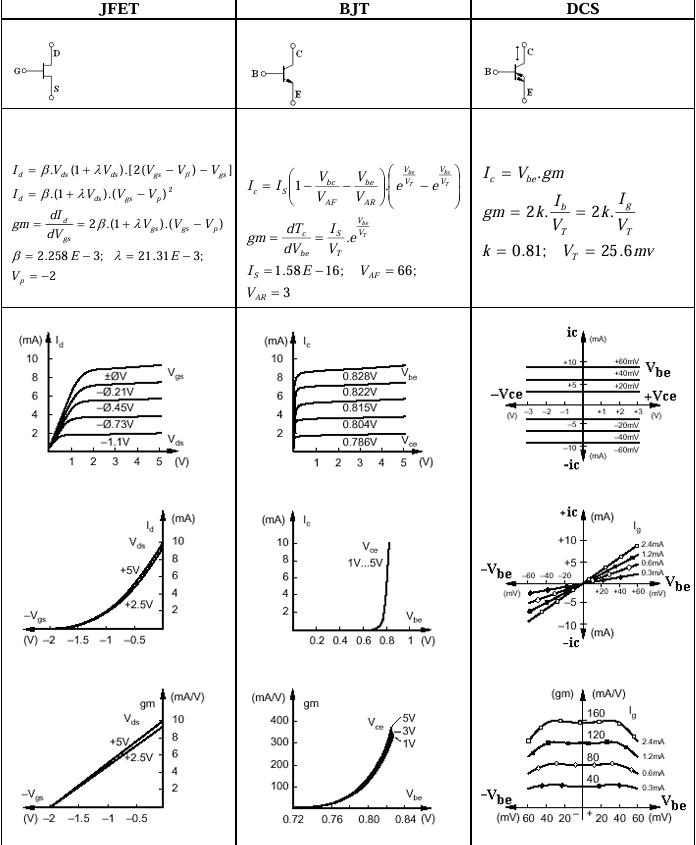
\includegraphics[width=1\linewidth]{Imagenes/4.13.png}
    \caption{Cortesía Burr-Brown Corp.}
    \label{fig:4.13}
\end{figure}
\textbf{Amplificador directo}
De igual manera que el tipo OTA-VFA, el TD puede operar como amplificador directo de ganancia controlada. El campo de aplicación relevante de esta aplicación es en muy alta frecuencia, como excitador de cargas con fuertes componentes capacitivas (Line Driver). En los párrafos siguientes se analiza de un modo general, su modo de operación en bajas frecuencias poniendo en evidencia sus características amplificadoras en cuatro cuadrantes, como lo muestra la fig \ref{fig:4.14}b, donde la ecuación de la recta de carga derivada de \ref{fig:4.14}a será para $R_{in}=1/g_m \ll R_e$:

\begin{equation}
v_{ce} = v_c - v_e =  i_c (R_c - R_e)
\label{eq:4.9}
\end{equation}
\begin{figure}[H]
    \centering
    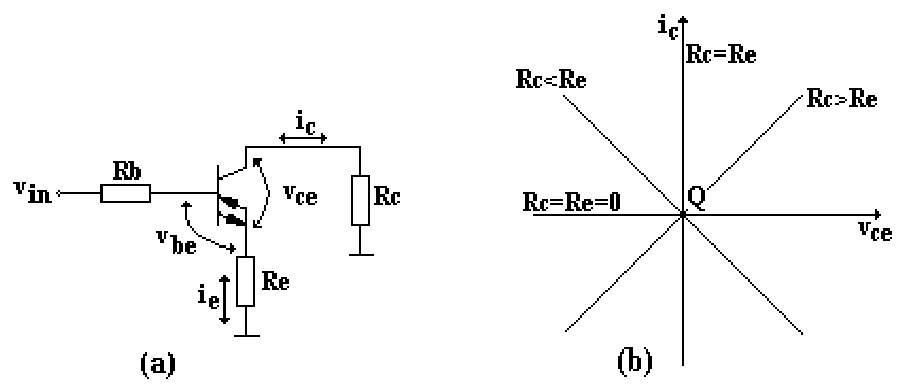
\includegraphics[width=0.75\linewidth]{Imagenes/4.14.png}
    \caption{}
    \label{fig:4.14}
\end{figure}

Luego, según muestra la fig. \ref{fig:4.14}b la pendiente de la recta de carga será positiva, negativa, infinita o nula, según sean los valores relativos de $R_c$ y $R_e$. El punto de operación en reposo ($Q$), coincidirá con el origen de coordenadas.

Si en cambio la señal $V_{in}$ tuviere componente de continua (la que no debe superar el rango de modo diferencial admitido), puede ocurrir cualquiera de las situaciones mostradas en la fig. \ref{fig:4.15}, según sea la polaridad de aquella y los valores relativos de las resistencias ya mencionadas.
\begin{figure}[H]
    \centering
    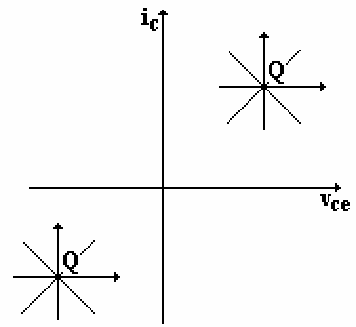
\includegraphics[width=0.5\linewidth]{Imagenes/4.15.png}
    \caption{}
    \label{fig:4.15}
\end{figure}
En general, las configuraciones simples o compuestas realizadas con transistores discretos clásicos, pueden también ser emuladas por el Transistor Diamante, más algunas que le son propias. No obstante siempre pueden ser analizadas por simple inspección.
\textbf{Emisor común}
Este modo de operación se corresponde con el esquema de la fig. \ref{fig:4.12} y se repite en la fig. \ref{fig:4.16}. De ellos se deducen las siguientes relaciones:

$$
v_0 = i_c \cdot R_c \quad \therefore \quad i_c = i_e = \frac{V_{in}}{R_e + \frac{1}{g_m}}
$$

\begin{equation}
A_v = \frac{V_0}{V_{in}} = \frac{R_c}{R_e + \frac{1}{g_m}} = \frac{\frac{R_c}{R_e}}{1 + \frac{1}{g_m \cdot R_e}}
\tag{4.10}
\end{equation}

Si se desprecia la resistencia de entrada en emisor, se obtiene la expresión clásica de la ganancia de tensión

\begin{equation}
R_e \gg \frac{1}{g_m} \quad \Rightarrow \quad A_v = \frac{R_c}{R_e}
\tag{4.11}
\end{equation}

Se obtiene máxima ganancia de tensión haciendo $R_e=0$

\begin{equation}
A_v = g_m \cdot R_c
\tag{4.12}
\end{equation}

La fig \ref{fig:4.16}c muestra la recta de carga para este último caso.
\begin{figure}[H]
    \centering
    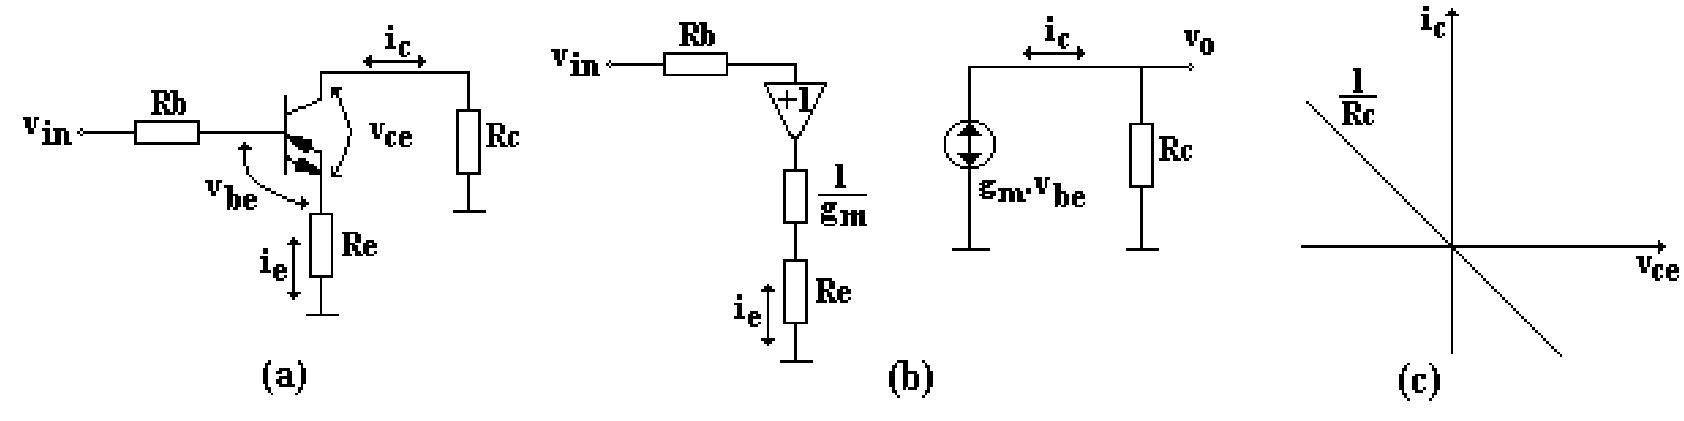
\includegraphics[width=0.95\linewidth]{Imagenes/4.16.png}
    \caption{}
    \label{fig:4.16}
\end{figure}
\textbf{Base común}
Esta configuración (fig \ref{fig:4.17}), genera las mismas funciones de transferencia que la anterior, excepto la inversión de fase entrada salida. En consecuencia la ganancia de tensión se expresa, según que la resistencia de emisor sea nula o no con alguna de las mostradas en (\ref{eq:4.13}).
\begin{figure}[H]
    \centering
    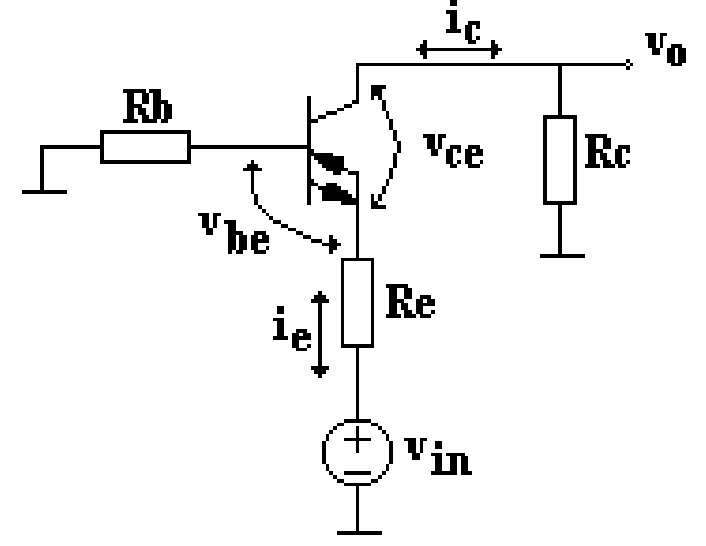
\includegraphics[width=0.5\linewidth]{Imagenes/4.17.png}
    \caption{}
    \label{fig:4.17}
\end{figure}
Esta configuración (fig \ref{fig:4.17}), genera las mismas funciones de transferencia que la anterior, excepto la inversión de fase entrada salida. En consecuencia la ganancia de tensión se expresa, según que la resistencia de emisor sea nula o no con alguna de las mostradas en (\ref{eq:4.13}).

\begin{equation}
A_v = \frac{-R_c}{R_e + \frac{1}{g_m}} \cong -\frac{R_c}{R_e}
\label{eq:4.13}
\end{equation}

$$
A_v \bigg|_{R_e=0} = -g_m \cdot R_c
$$
\textbf{Colector común (Buffer)}
El Transistor Diamante, permite configurar dos esquemas diferentes para la función buffer. El de la fig. \ref{fig:4.18}, muestra una de ellas, que se corresponde con la conexión clásica.
\begin{figure}[H]
    \centering
    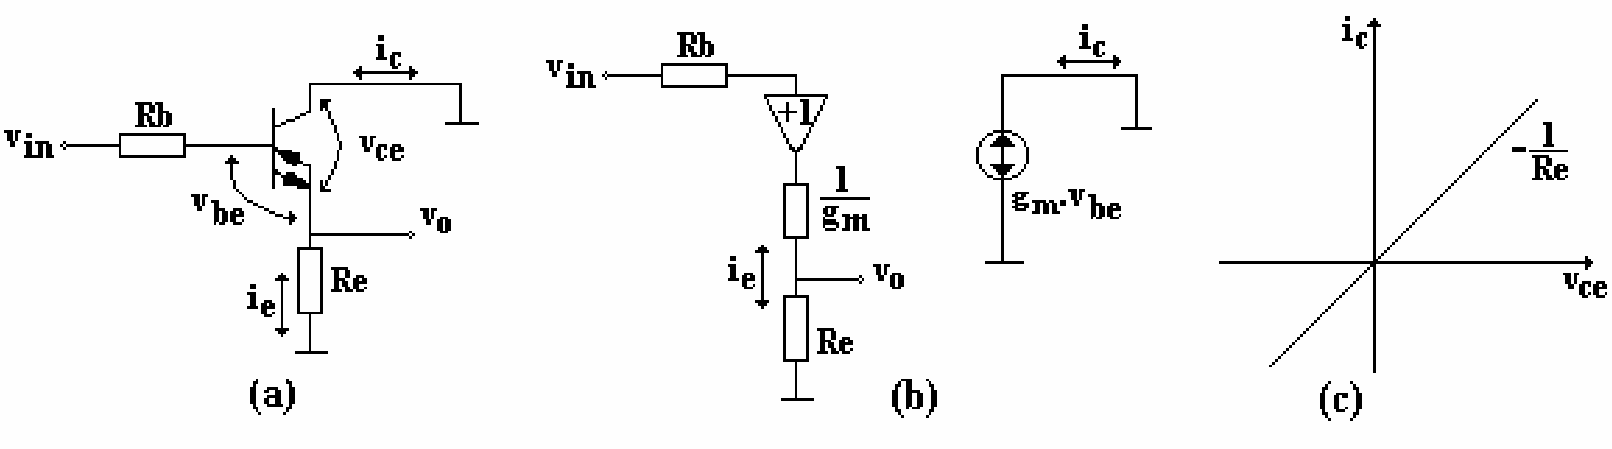
\includegraphics[width=1\linewidth]{Imagenes/4.18.png}
    \caption{}
    \label{fig:4.18}
\end{figure}
La ganancia de tensión es:

$$
v_0 = i_e \cdot R_e \quad \therefore \quad i_e = \frac{V_{in} - V_0}{\frac{1}{g_m}}
$$

\begin{equation}
A_v = \frac{V_0}{V_{in}} = \frac{1}{1 + \frac{1}{g_m \cdot R_e}} \cong 1
\tag{4.14}
\end{equation}

La fig. \ref{fig:4.19} muestra otra posibilidad de configurar un amplificador buffer duplicando la corriente en la carga. Esta conexión es propia del Transistor Diamante y mejora la función separadora del circuito anterior.
\begin{figure}[H]
    \centering
    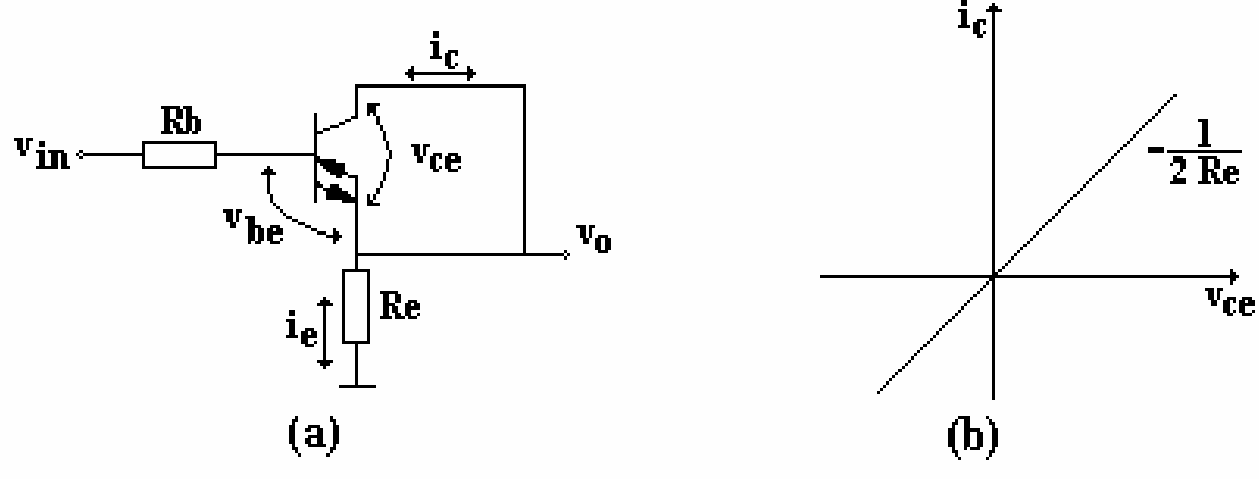
\includegraphics[width=0.75\linewidth]{Imagenes/4.19.png}
    \caption{}
    \label{fig:4.19}
\end{figure}
\begin{equation}
v_0 = 2 \cdot i_e \cdot R_e
\tag{4.15}
\end{equation}

Relacionando 4.14 y 4.15 se obtiene:

\begin{equation}
A_v = \frac{1}{1 + \frac{1}{2 \cdot R_e \cdot g_m}} \cong 1
\tag{4.16}
\end{equation}
\textbf{Configuraciones realimentadas}
La versión comercial del TD (OPA660) incluye en el mismo chip, un Buffer, que entre otras aplicaciones, permite configurar un amplificador integrado realimentado por corriente (CFA), por la conexión en cascada de ambos como muestra la figura \ref{fig:4.20}a, donde el conjunto realimentado por red exterior ($R_1$, $R_2$), configura un no inversor.

Si además se buferea la unión del divisor resistivo al emisor con un segundo Buffer (fig \ref{fig:4.20}b), resulta un amplificador operacional clásico.
\begin{figure}[H]
    \centering
    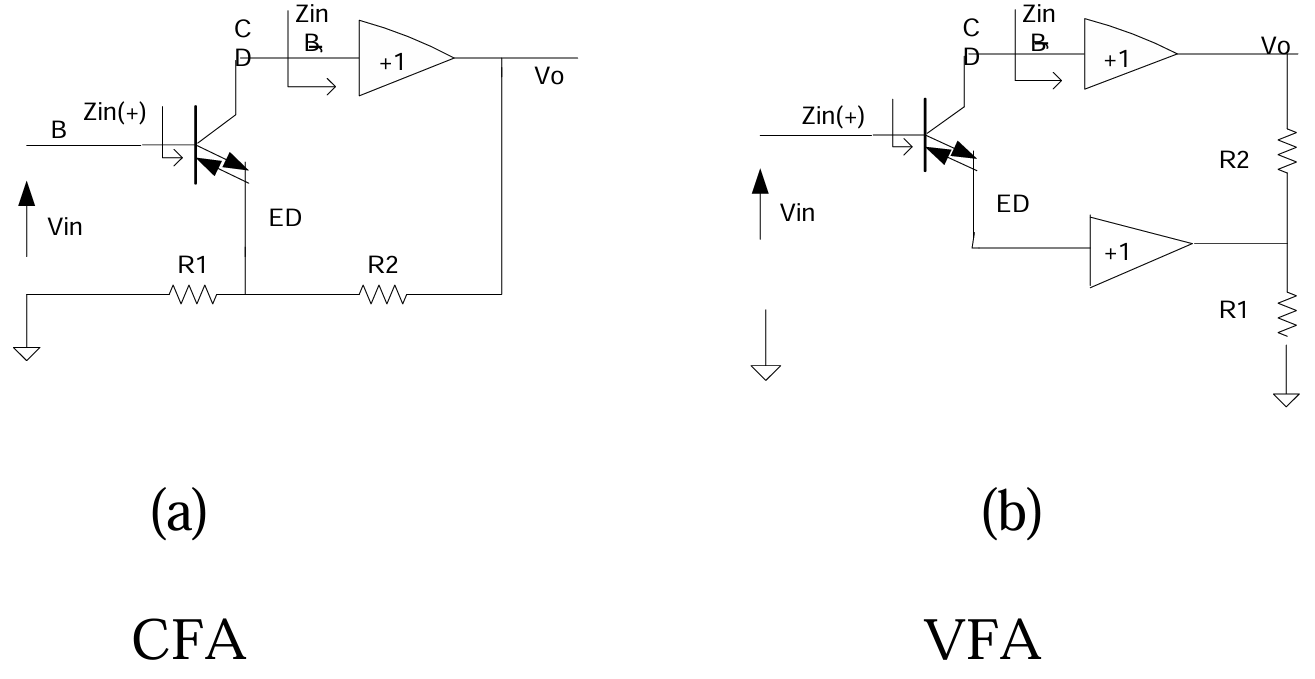
\includegraphics[width=0.75\linewidth]{Imagenes/4.20.png}
    \caption{}
    \label{fig:4.20}
\end{figure}